
\chapter{Methods and fabrication.}

\section{Quantum dot growth}

The QD source was grown by molecular beam epitaxy (MBE). MBE allows deposition
of various semiconductor layers with atomic precision of the layer height. The
QD sample used in this project had an embedded planar distributed bragg
reflector cavity to optimise the vertical emission mode from the QDs. The index
schematic of this structure is shown in Figure \ref{fig:planar_cav}. The
structure was grown on a GaAs substrate. Each reflector mirror repeat was made
by a layer of GaAs and a layer of AlAs. The cavity was created by placing twelve
mirror repeats of size $\lambda/4n$ where $\lambda = 910nm$ and $n$ is the
refractive index of the material. For GaAs this is 3.59 and for AlAs this is
2.97. Then a $2\lambda/n$ spacing of GaAs was grown with an embedded InAs layer
0.5nm thick. Finally two mirror repeats were grown on top. The emission
wavelength typically in the range 890 to 950nm.

\begin{figure}[h!] \begin{center}
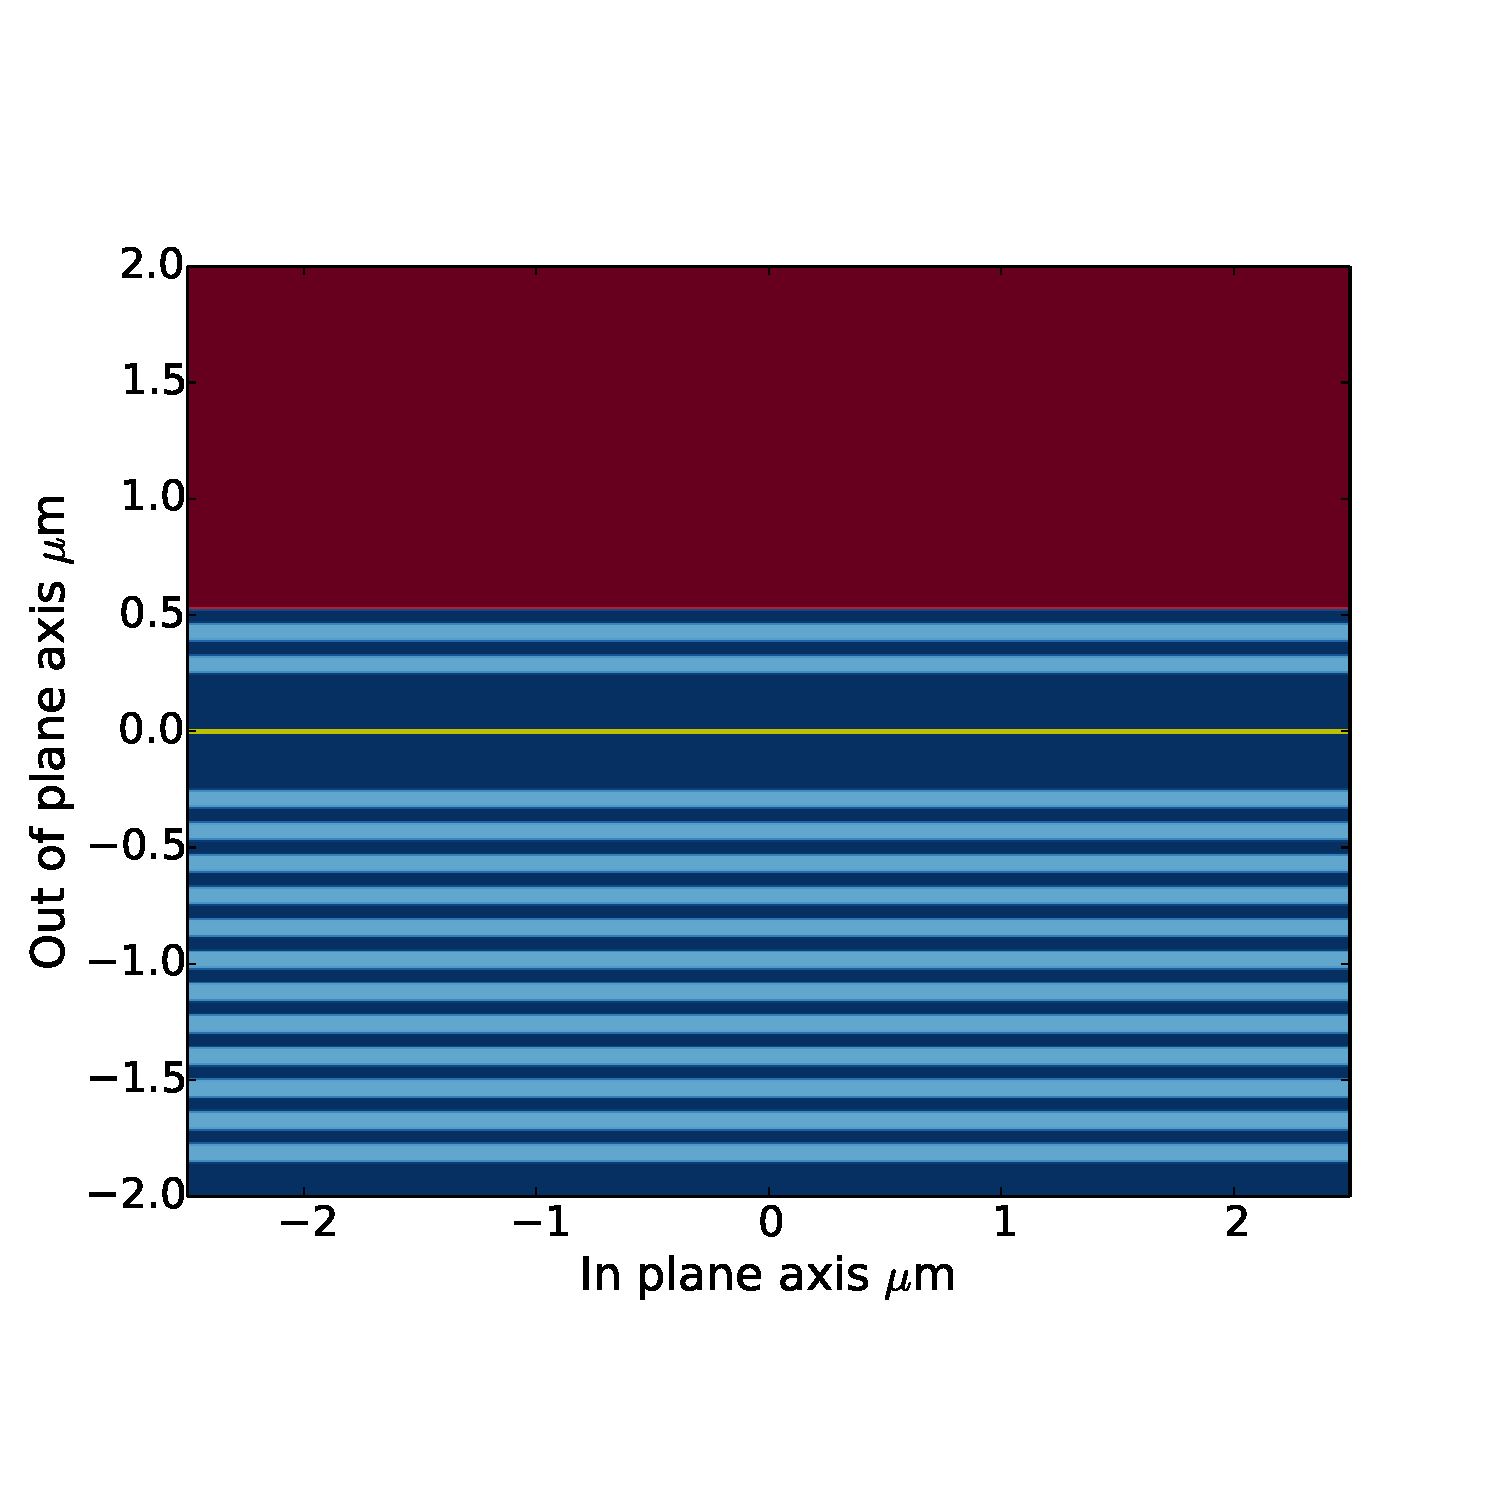
\includegraphics[width=0.8\textwidth]{images/qd_layers.pdf} \end{center}
\caption{Index structure of the grown QD sample The red section is air with a
refractive index of 1 and the alternating blue layers are GaAs and AlAs.}
\label{fig:planar_cav} \end{figure}

\section{Waveguide fabrication and characterisation}

The SiON waveguide chip device was fabricated by plasma enhanced chemical vapour
deposition to define a layer of SiO$_2$ undercladding and SiON core on a silicon
substrate. Electron-beam lithography and reactive ion etching were used to
define the SiON core profile before finally an SiO$_2$ overclad layer was
defined. During the lithography process arbitrary waveguide shapes can be
imparted onto the device. These can be S-bends, directional couplers and/or Mach
Zehnder interferometers. Once the fabrication of the device was complete the
chips were then characterised. In this project the index of the core was 1.55
and the cladding was 1.51, the waveguide size was 1.6um to keep the guide single
mode.

\begin{figure}[h!] \begin{center}
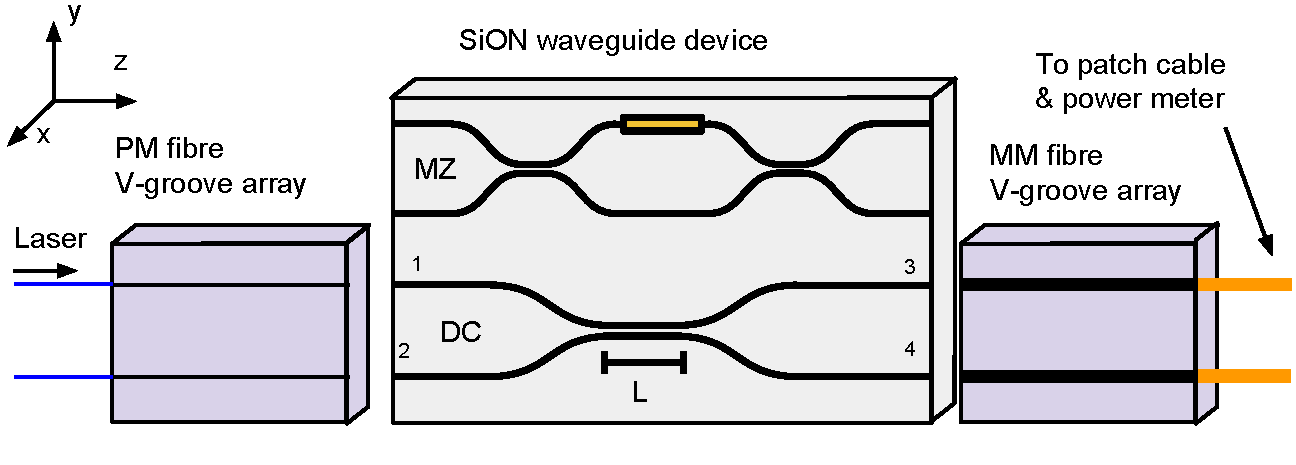
\includegraphics[width=0.8\textwidth]{images/wg_char.pdf} \end{center}
\caption{Schematic of waveguide characterisation experiment.} \label{fig:6axis}
\end{figure}

Two V-groove arrays each were mounted on 6 axis stages which allowed precise
alignment of the V-grooves to the side of the SiON waveguide chip. The V-grooves
are commercially available arrays of fibres. A substrate is patterned with an
array of V shaped grooves into which optical fibres are planted and sealed. This
experiment layout is shown in Figure \ref{fig:6axis}. The one of the PM fibres
injects laser light into port 1. The laser used was a tuneable Fabry Perot
cavity laser emitting in the range 890 to 935nm. This light propagates through
the chip and is collected by the multimode V-groove array at ports 3 and 4 and
is then sent to power meters. This allows the calculation of the coupling ratio
of the directional couplers. Injecting light into both port 1 and then 2 allows
calculation of the coupling ratio which is independant of the coupling loss. The
coupling ratio in the lossless case is as follows:

\begin{equation} r  = \frac{P_{13}}{I} = \frac{P_{24}}{I} \end{equation}

Where $P_{ij}$ is the power measured at port $j$ when light is injected into
port $i$. The parameter $I$ is the injected laser power. The conservation of
power in the lossless case allows:

\begin{equation} I = P_{13}+P_{14} = P_{23}+P_{24} \end{equation}

and

\begin{equation}\label{eqn:p1} P_{13}+P_{24} = Ir \end{equation}\label{eqn:p2}
\begin{equation} P_{14}+P_{23} = I(1-r) \end{equation}

However since there exists coupling loss and at each port, given by $l_i$, the
powers measured at each port become

\begin{equation} P^{'}_{ij} = l_i l_j P_{ij} \end{equation}

Then by taking a power ratio the losses can be canceled

\begin{equation} \frac{ P^{'}_{13} P^{'}_{24} }{ P^{'}_{14} P^{'}_{23} } =
\frac{ l_1 l_3 P_{13} l_2 l_4 P_{24} }{ l_1l_4P_{14}l_2l_3P_{23} }
\end{equation}

From Equation \ref{eqn:p1} and \ref{eqn:p2} this gives an expression for the
coupling ratio

\begin{equation} \left(\frac{r}{1-r}\right)*2 = \frac{P^{'}_{13}
P^{'}_{24}}{P^{'}_{14} P^{'}_{23}} \end{equation}

Rearranging to give

\begin{equation} r = \frac{\sqrt{\frac{P^{'}_{13} P^{'}_{24}}{P^{'}_{14}
P^{'}_{23}}}}{1+ \sqrt{\frac{P^{'}_{13} P^{'}_{24}}{P^{'}_{14} P^{'}_{23}}}}
\end{equation}

This allows an accurate calculation of the coupling ratio which is independant
of any coupling or alignment losses.

In order to characterise the MZIs a very similar experiment was performed except
that the powers were recorded as a voltage was applied to the heater. Then the
coupling ratio vs heater voltage was recorded. This shows how well the MZI can
switch light between the two ports, this is quantified with by calculating the
visibility.

\begin{equation} V = 100 \frac{r_{max} - r_{min}}{r_{max} + r_{min}}
\end{equation}

This percentage shows the maximum switching capability of the MZI. A visiblity
of 100\% means that all of the light can be coupled to one port, with no light
in the other. A visiblity of 80\% means that, at best, the MZI will send only
80\% of the light to one port and 20\% to the other.

\section{Hybrid chip}


\subsection{Simulations and design}

\begin{figure}[h!] \begin{center}
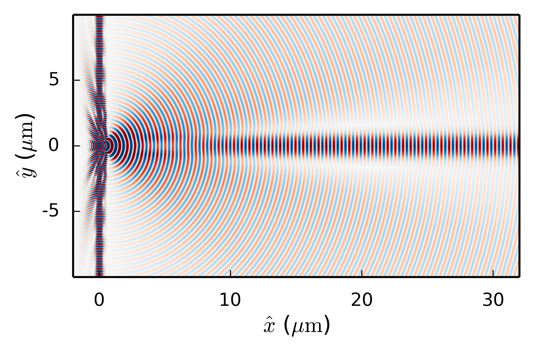
\includegraphics[width=0.8\textwidth]{images/sim.png} \caption{Finite difference
time domain simulation of a QD dipole emitting in a cavity and the emission
being guided by the SiON core.} \label{fig:sim} \end{center} \end{figure}

As described in Chapter 2 the characteristics of the device were simulated by
using the finite difference time domain package MEEP \cite{oskooi2010meep,
mandelshtam1997harmonic}. A $\hat{z}$ oriented dipole emitter was placed in the
centre of the cavity spacer aligned to the centre of the waveguide. A perfectly
matched layer was placed at the edges of the simulation domain to absorb all
light and prevent unwanted reflections. The $\hat{z}$ component of the electric
field is shown in Figure \ref{fig:sim}. There is a clear emission pattern along
the waveguide core. The efficiency of this device was also determined
theoretically. A bounding box which records the Fourier transformed fields was
placed at the edge of the domain and just inside the perfectly matched layer.

From this bounding box the total power spectrum is recorded when the system is
excited with a short Gaussian pulse. Another flux plane is placed across the
waveguide. The waveguide core size was 1.6 $\mu \mathrm{m}$ and the far field
propagating mode has a spatial $1/e$ width of 1.88 $\mu \mathrm{m}$ which was
chosen as the size of the waveguide flux plane. It is placed sufficiently far
from the surface of the III-V so that only the waveguide propagating mode is
measured. Taking the ratio of the light propagating in the waveguide to the
total in the bounding box gives the efficiency of the hybrid collection system.
At the centre of the cavity wavelength the efficiency is 2.8\%. For a QD
emitting into free space with no cavity a collection of 0.5\% can be expected
into a 0.5 NA objective. When the QD is in a cavity the efficiency can rise to
7\% depending on the number of mirror repeats and the numerical aperature of the
collection objective. For the device presented here the numerical aperature of
the waveguide is 0.35 and the III-V sample has a distributed bragg reflector
cavity with 12 repeats below the QD layer and 2 repeats above. This efficiency
of 2.8\% is almost exactly in line with what has previously been estimated for
free space collection with the same NA and same number of repeats
\cite{bennett2006single}.

\subsection{Packaging}

\begin{figure}[h!] \begin{center}
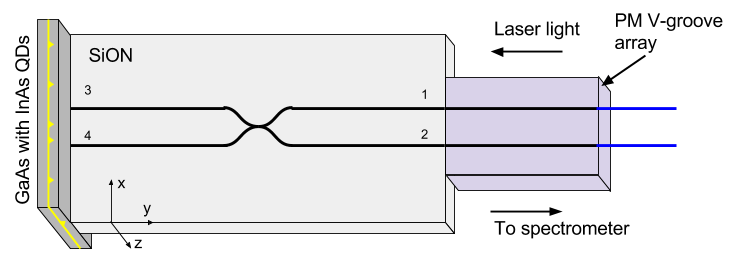
\includegraphics[width=0.8\textwidth]{images/hyb_basic.png} \caption{Schematic
of a hybrid device. A III-V chip with embedded quantum dots is bonded to an SiON
waveguide chip such that the single photons from the QDs are routed through the
waveguides.} \label{fig:hyb_basic} \end{center} \end{figure}

The III-V chip was bonded orthogonally to the SiON waveguide chip as shown in
Figure \ref{fig:hyb_basic} by optical UV cured adhesive. This allows the surface
emission of the III-V chip to be collected by the waveguides. The DC is needed
to allow seperate fibres for laser delivery and for QD light collection. The
laser light is delivered through port 1. The laser power is split by the DC and
will excite QDs at the ends of ports 3 and 4. This QD is collected by the
waveguides and will be split by the DC and sent to ports 1 and 2. That which
reaches port 2 is sent to a spectrometer equipped with a silicon charged-coupled
device. During experiments the entire device was kept at 4K. Throughout this
project the laser used was above the bandgap of GaAs, resonant or quasi-resonant
excitation was not used. The device shown in Figure \ref{fig:hyb_basic} is
useful only to check the emission of the QD into the waveguide, no on-chip
quantum operations can take place because all the available waveguides are used
for excitation and collection. In the next chapter a more sophisticated device
with an on-chip MZI will be discussed.

\section{Single photon statistics}

To verify the single photon nature of the QD emission a Hanbury Brown and Twiss
experiment must be performed. The second order correlation function
$g^{(2)}(\tau)$, as explained in Chapter 1, is measured by splitting a stream of
photons by a DC or beamsplitter. Both streams are then sent to avalanche
photodiodes (APDs) where the arrival time of each photon is measured. One APD
starts a clock and the other stops it. One APD is delayed by some time $\tau$ in
order to measure negative correlation values. An absence of hits at time $\tau =
0$ implies single photon emission.
